\begin{exercise}
      {ID-126b94e5583f1b4e31636a0353fe11814c14a4dd}
      {Pendel}
  \ifproblem\problem
    Wenn man ein Pendel \sicm{80} zur Seite auslenkt, hängt das Gewicht \sicm{25}
    höher als in Ruhelage. Wie lang ist das Pendel?
    \begin{center}
      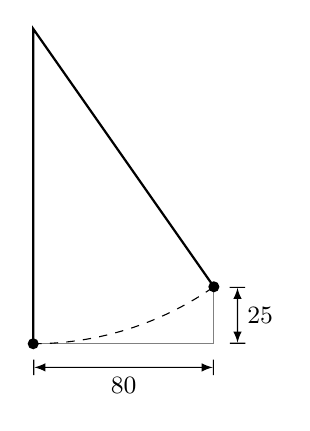
\begin{tikzpicture}
        % unten
        \coordinate (A) at (270:4cm);
        % oben
        \coordinate (B) at (0, 0);
        % rechts
        \coordinate (C) at (305:4cm);
        % Schnittpunkt der Hilfslinien
        \coordinate (D) at (intersection of C--[yshift=-10cm]C and A--[xshift=10cm]A);
        % Hilfslinien
        \draw[draw=white!50!black] (A) -| (C);
        % das Pendel
        \draw[line width=0.8pt] (A) -- (B) -- (C);
        % Kreislinie
        \draw[style=dashed] (A) arc (270:305:4cm);
        % Gewichte
        \fill (A) circle (2pt);
        \fill (C) circle (2pt);
        % Masse
        \draw[|<->|, >=latex] ([yshift=-3mm]A) -- node[below]{{\small\sicm{80}}} ([yshift=-3mm]D);
        \draw[|<->|, >=latex] ([xshift=3mm]C) -- node[right]{{\small\sicm{25}}} ([xshift=3mm]D);
      \end{tikzpicture}
    \end{center}
  \fi
  \ifoutline\outline
    \begin{center}%
      \begin{tikzpicture}
        % unten
        \coordinate (A) at (270:4cm);
        % oben
        \coordinate (B) at (0, 0);
        % rechts
        \coordinate (C) at (305:4cm);
        % Projektion auf die y-Achse
        \path (C) -| coordinate (E) (A);
        % Hilfslinien und Punkt D
        \draw[draw=white!50!black] (A) -| coordinate (D) (C);
        % das Pendel
        \draw[line width=0.8pt] (A) -- (B) -- (C);
        % Kreislinie
        \draw[style=dashed] (A) arc (270:305:4cm);
        % Gewichte
        \fill (A) circle (2pt);
        \fill (C) circle (2pt);
        % fehlende Kathete
        \draw[draw=white!50!black] (C) -- (E);
        % rechter Winkel
        \draw[draw=white!50!black] ([xshift=5mm]E) arc[start angle=0, end angle=90, radius=5mm];
        \fill[fill=white!50!black] ([shift={(45:2.6mm)}]E) circle[radius=1.25pt];
        % Beschriftung
        \draw[|<->|, >=latex] ([yshift=-3mm]A) -- node[below]{$x$} ([yshift=-3mm]D);
        \draw[|<->|, >=latex] ([xshift=3mm]C) -- node[right]{$y$} ([xshift=3mm]D);
        \path (E) -- node[rotate=90, above]{$\ell-y$} (B);
        \path (B) -- node[above right]{$\ell$} (C);
        % Gleichungen
        \node[right] at (4, -2)
        {%
          \begin{minipage}{4cm}
            \setlength{\abovedisplayskip}{0pt}%
            \begin{equation*}
              \ell^2=x^2+(\ell-y)^2
            \end{equation*}
          \end{minipage}%
        };
      \end{tikzpicture}%
    \end{center}
  \fi
  \ifoutcome\outcome
    Das Pendel ist \sicm{140.5} lang.
  \fi
\end{exercise}
